\section{}

% ================== Freq vs Time =====================
\begin{figure}[htbp]
    \centering
    \vspace{-0.5em}
    \begin{subfigure}[b]{\textwidth}
        \centering
        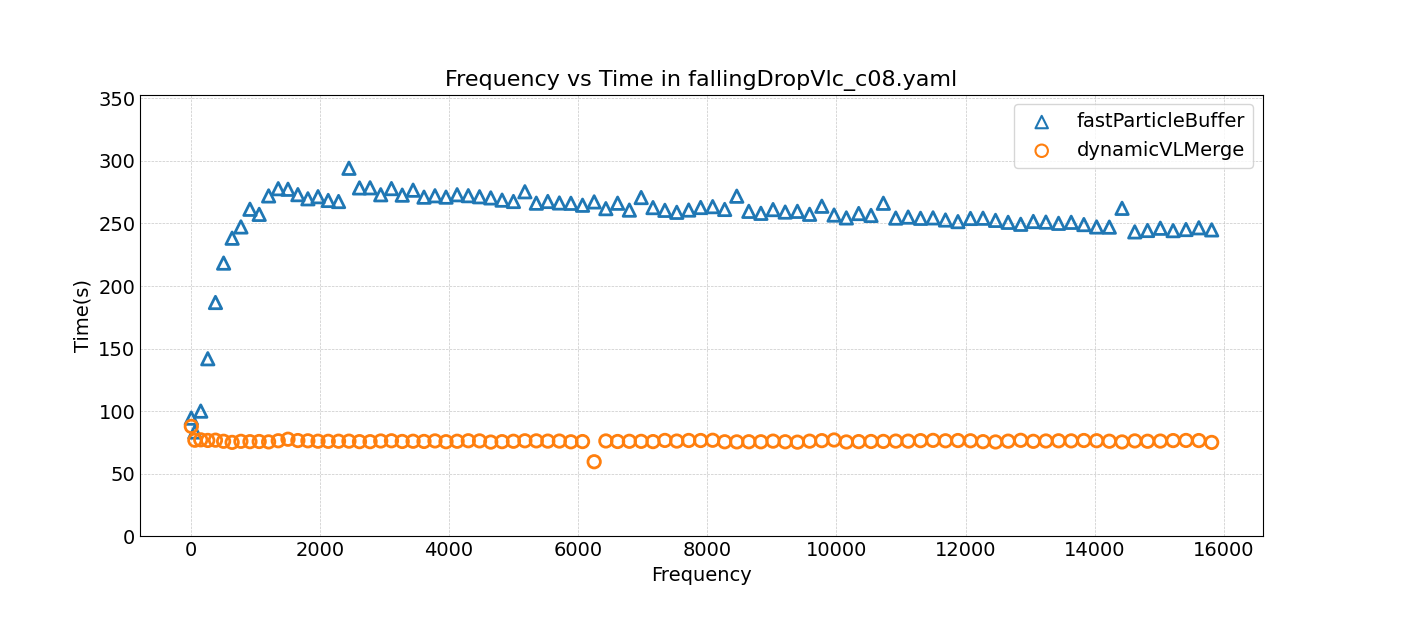
\includegraphics[width=0.9\linewidth]{graphs/fallingDrop/normalExperiments/freq/vlcc08.png}
        \vspace{-0.5em}
        \caption{\scriptsize Falling Drop vlc\_c08}
        \label{fig:vlcc08fallingDrop}
    \end{subfigure}

    \begin{subfigure}[b]{\textwidth}
        \centering
        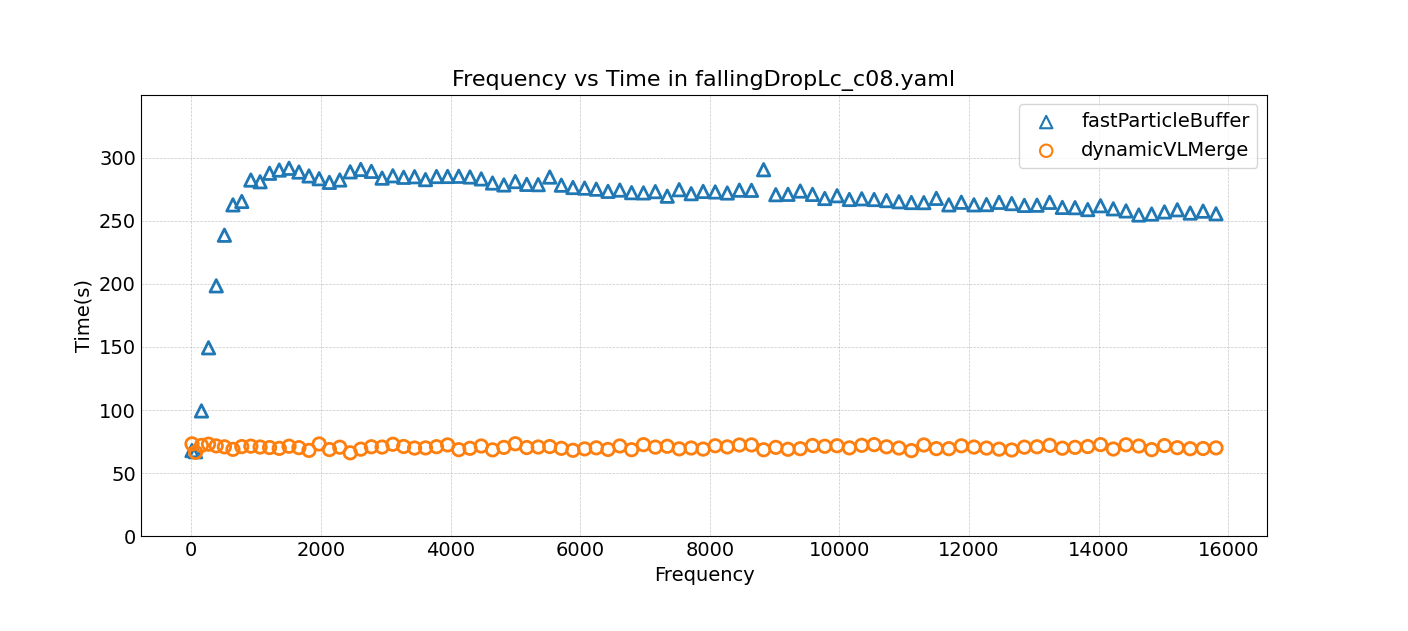
\includegraphics[width=0.9\linewidth]{graphs/fallingDrop/normalExperiments/freq/lcc08.png}
        \vspace{-0.5em}
        \caption{\scriptsize Falling Drop lc\_c08}
        \label{fig:lcc08explodingLiquid}
    \end{subfigure}

    \begin{subfigure}[b]{\textwidth}
        \centering
        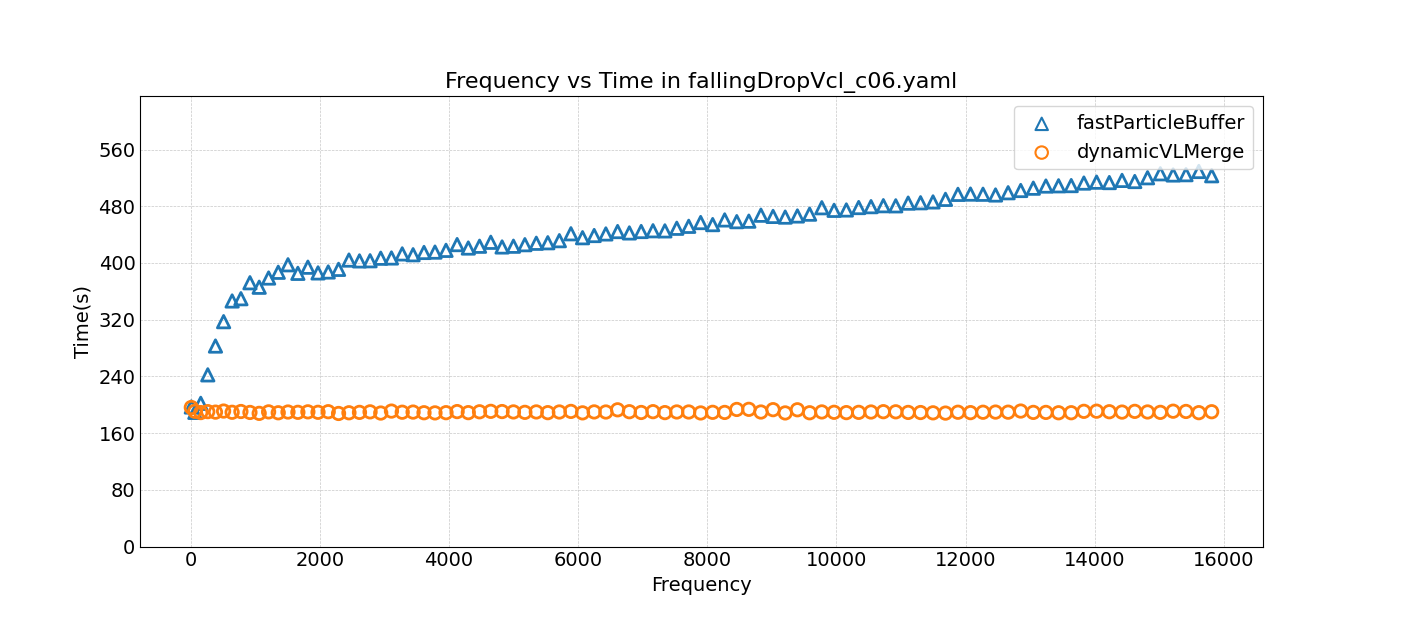
\includegraphics[width=0.9\linewidth]{graphs/fallingDrop/normalExperiments/freq/vclc06.png}
        \vspace{-0.5em}
        \caption{\scriptsize Falling Drop vcl\_c06}
        \label{fig:vclc06constantVelocityCube}
    \end{subfigure}

    \vspace{1em}
    \caption{Comparison of Frequency vs Time for Falling Drop Experiments}
    \label{fig:mainFallingDrop}
\end{figure}


\begin{figure}[htbp]
    \centering
    \vspace{-0.5em}
    \begin{subfigure}[b]{\textwidth}
        \centering
        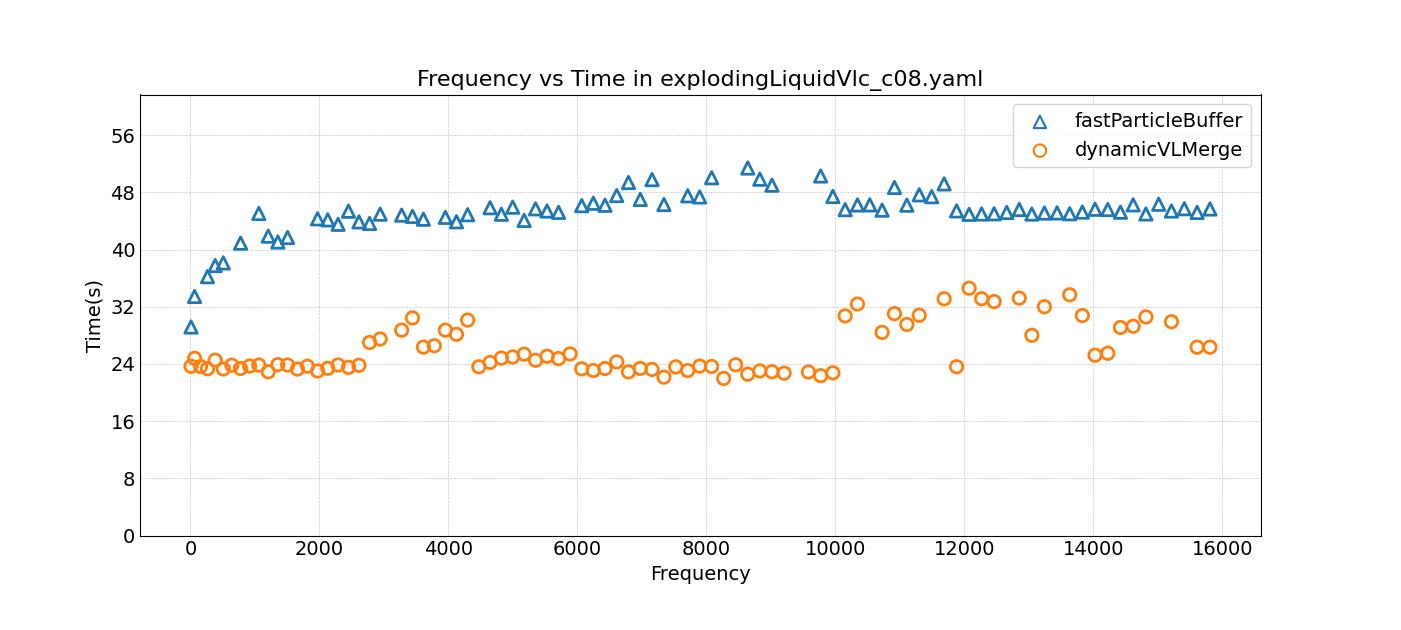
\includegraphics[width=0.9\linewidth]{graphs/explodingLiquid/normalExperiments/freq/vlcc08.png}
        \vspace{-0.5em}
        \caption{\scriptsize Exploding Liquid vlc\_c08}
        \label{fig:vlcc08explodingLiquid}
    \end{subfigure}

    \begin{subfigure}[b]{\textwidth}
        \centering
        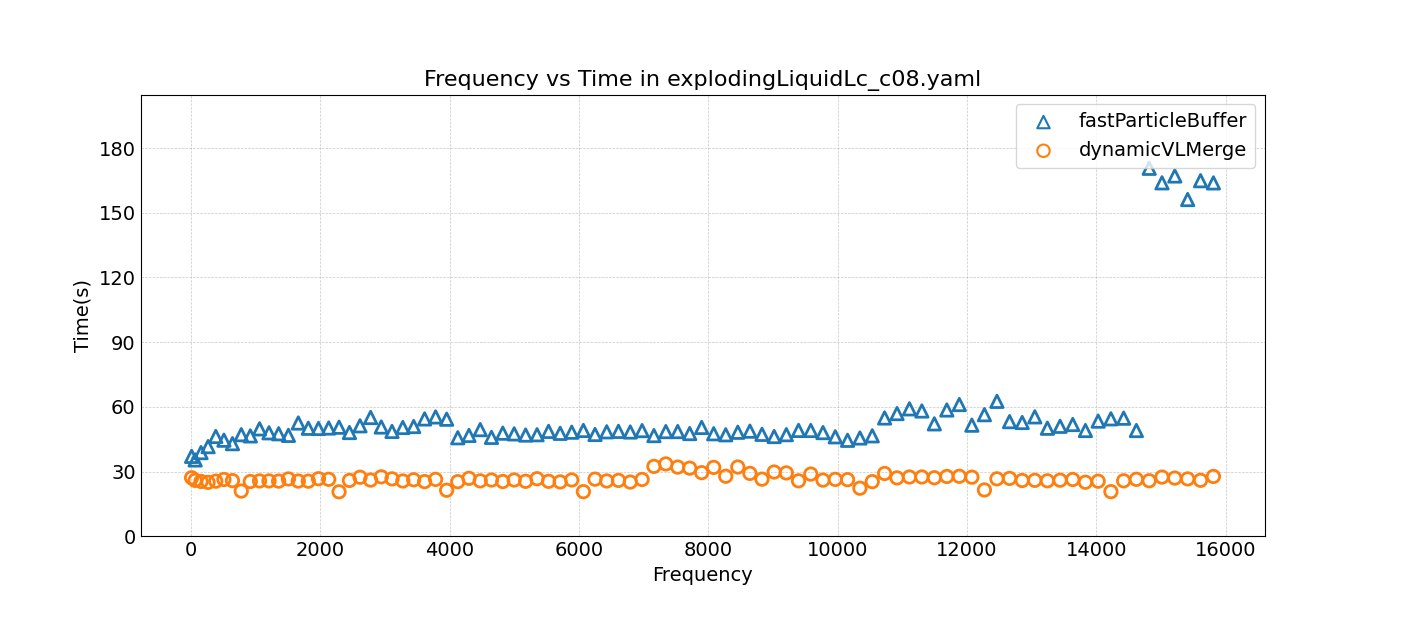
\includegraphics[width=0.9\linewidth]{graphs/explodingLiquid/normalExperiments/freq/lcc08.png}
        \vspace{-0.5em}
        \caption{\scriptsize Exploding Liquid lc\_c08}
        \label{fig:lcc08explodingLiquid}
    \end{subfigure}

    \begin{subfigure}[b]{\textwidth}
        \centering
        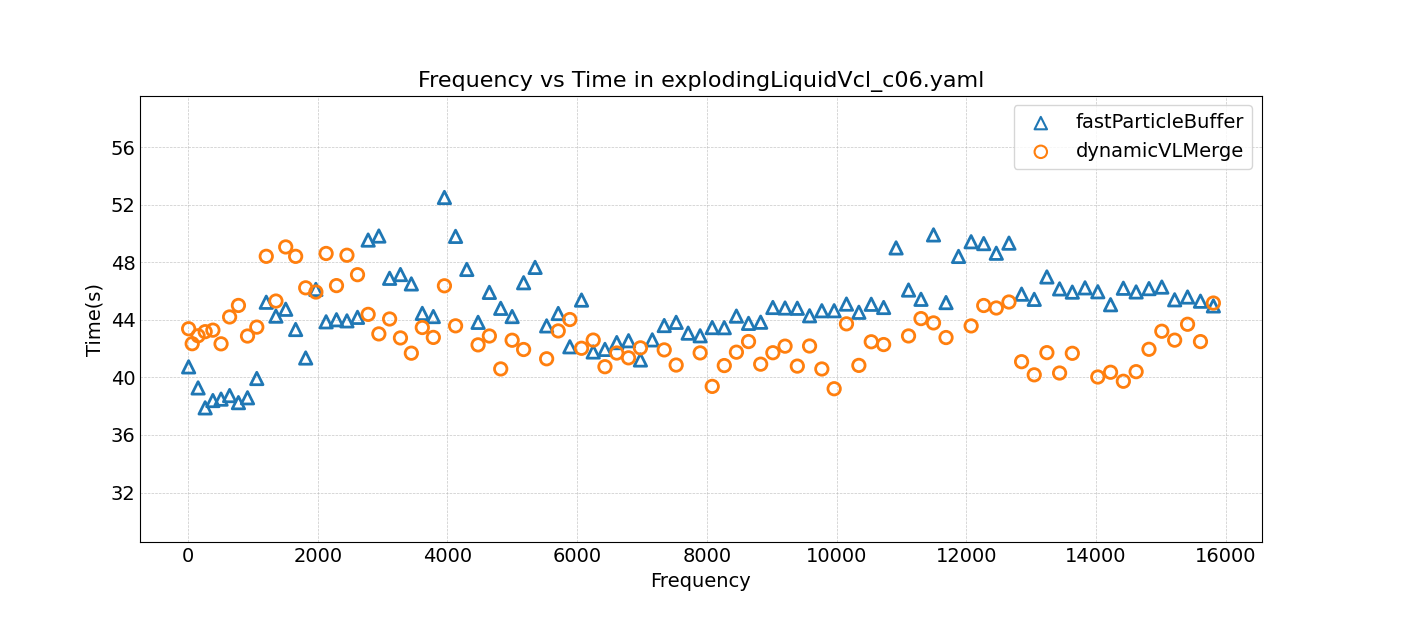
\includegraphics[width=0.9\linewidth]{graphs/explodingLiquid/normalExperiments/freq/vclc06.png}
        \vspace{-0.5em}
        \caption{\scriptsize Exploding Liquid vcl\_c06}
        \label{fig:vclc06explodingLiquid}
    \end{subfigure}

    \vspace{1em}
    \caption{Comparison of Frequency vs Time for Exploding Liquid Experiments}
    \label{fig:mainExplodingLiquid}
\end{figure}


\begin{figure}[htbp]
    \centering
    \vspace{-0.5em}
    \begin{subfigure}[b]{\textwidth}
        \centering
        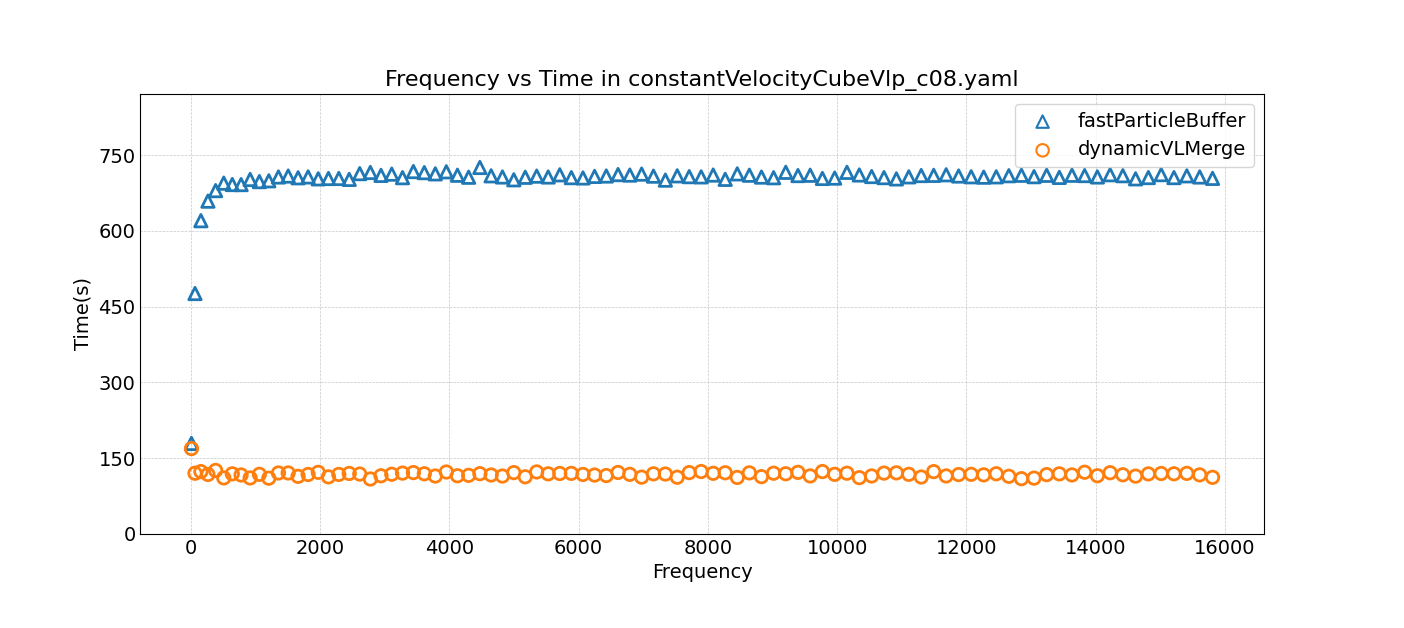
\includegraphics[width=0.9\linewidth]{graphs/constantVelocityCube/normalExperiments/freq/vlpc08.png}
        \vspace{-0.5em}
        \caption{\scriptsize Constant Velocity Cube vlp\_c08}
        \label{fig:vlpc08constantVelocityCube}
    \end{subfigure}

    \begin{subfigure}[b]{\textwidth}
        \centering
        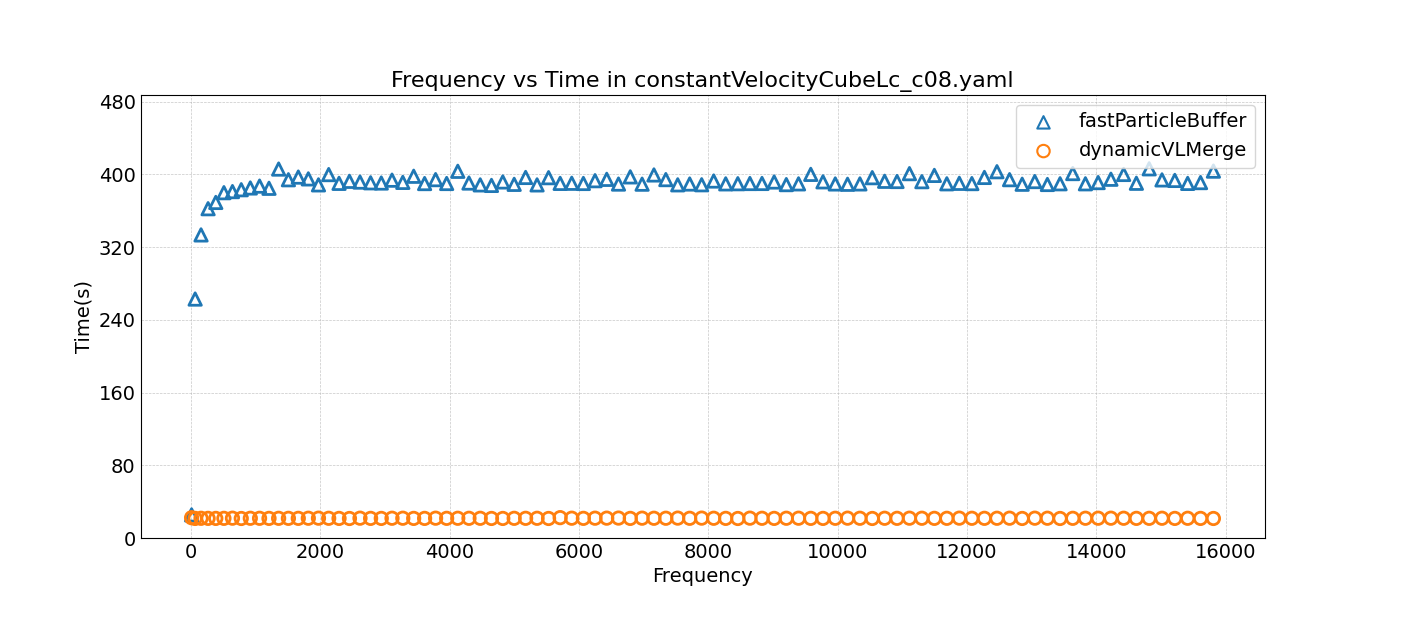
\includegraphics[width=0.9\linewidth]{graphs/constantVelocityCube/normalExperiments/freq/lcc08.png}
        \vspace{-0.5em}
        \caption{\scriptsize Constant Velocity Cube lc\_c08}
        \label{fig:lcc08constantVelocityCube}
    \end{subfigure}

    \begin{subfigure}[b]{\textwidth}
        \centering
        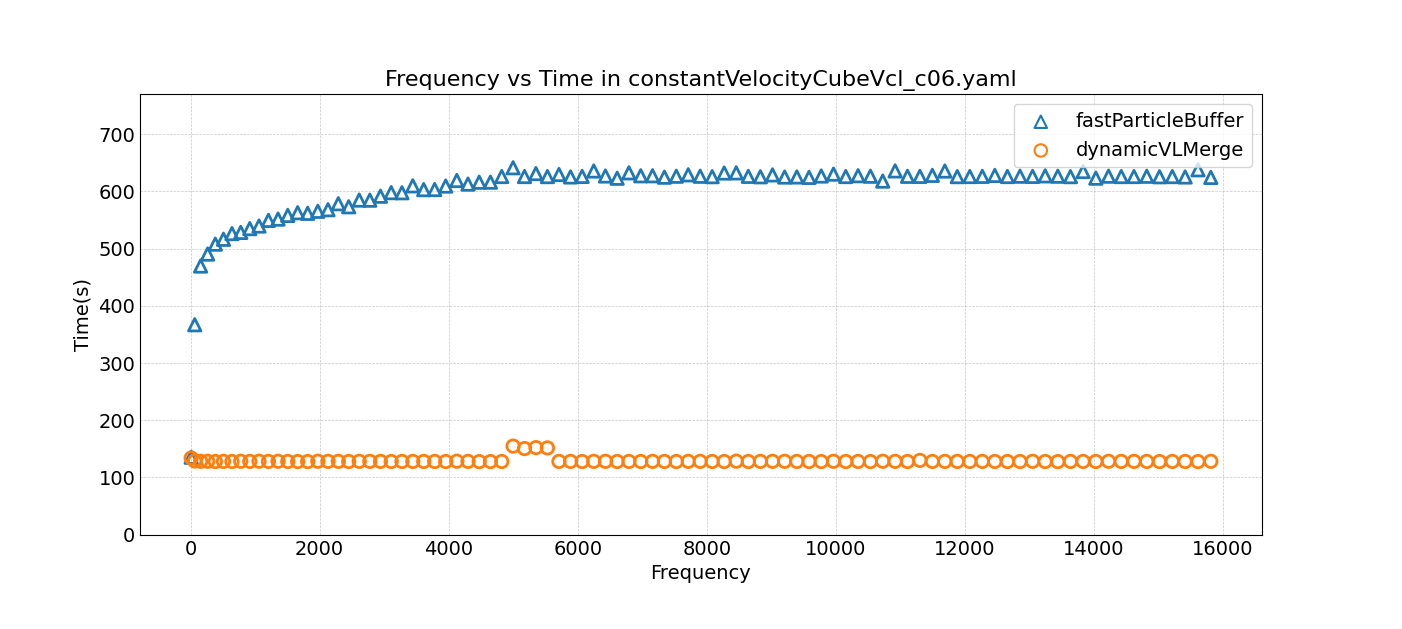
\includegraphics[width=0.9\linewidth]{graphs/constantVelocityCube/normalExperiments/freq/vclc06.png}
        \vspace{-0.5em}
        \caption{\scriptsize Constant Velocity Cube vcl\_c06}
        \label{fig:vclc06constantVelocityCube}
    \end{subfigure}

    \vspace{1em}
    \caption{Comparison of Frequency vs Time for Constant Velocity Cube Experiments}
    \label{fig:mainConstantVelocityCube}
\end{figure}

% ======================================================


% =====================Compute Inter vs Remainder Traversal Exploding Liquid=================================

\begin{figure}[htbp]
    \centering
    \vspace{-0.5em}
    \begin{subfigure}[b]{\textwidth}
        \centering
        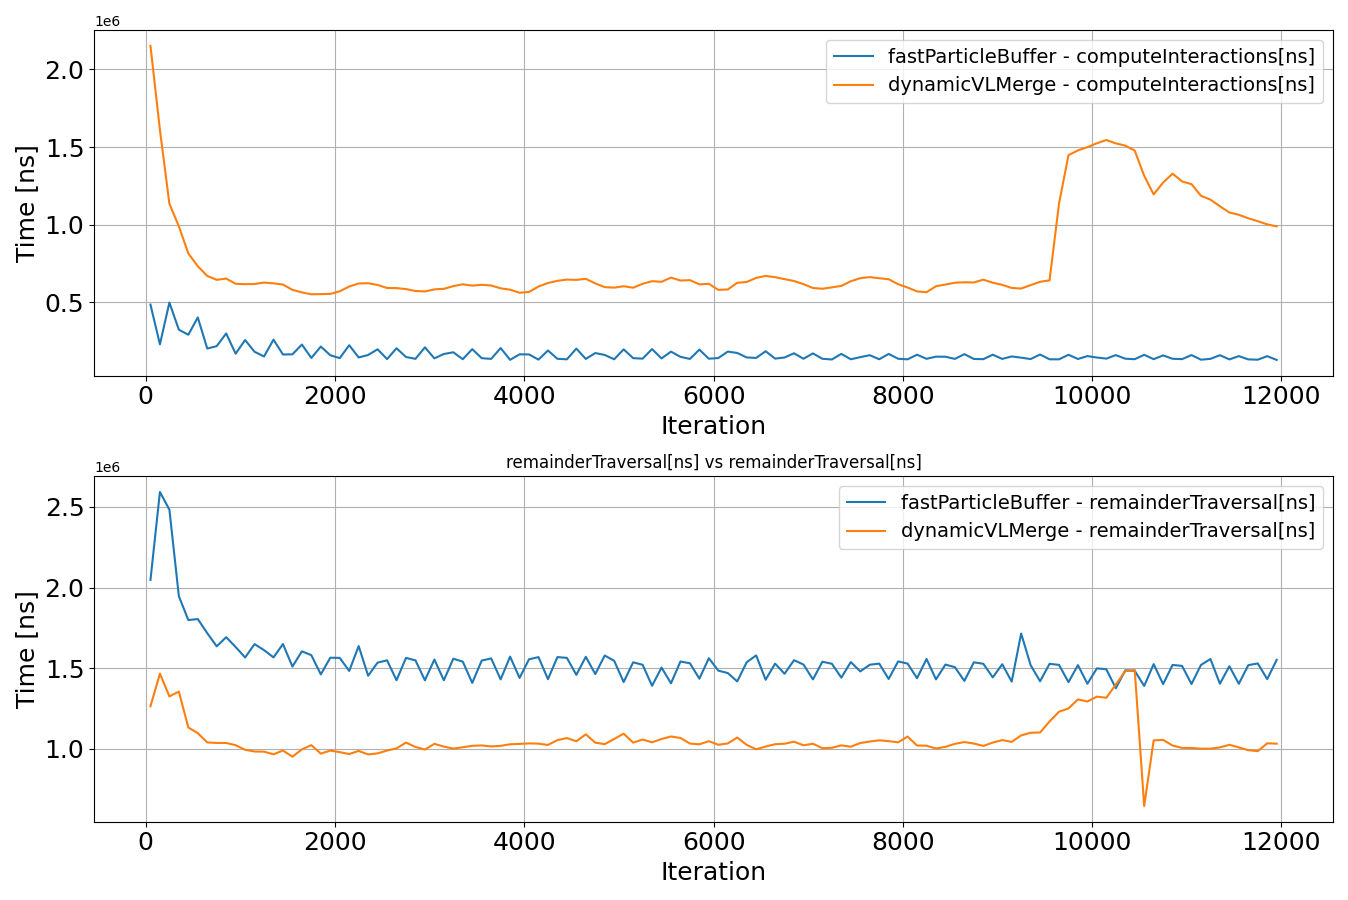
\includegraphics[width=0.9\linewidth]{graphs/explodingLiquid/normalExperiments/freq/vclc0_6inter.png}
        \vspace{-0.5em}
        \caption{\scriptsize Exploding Liquid Vcl\_c06}
        \label{fig:explodingLiquid_vclc0_6inter}
    \end{subfigure}

    \begin{subfigure}[b]{\textwidth}
        \centering
        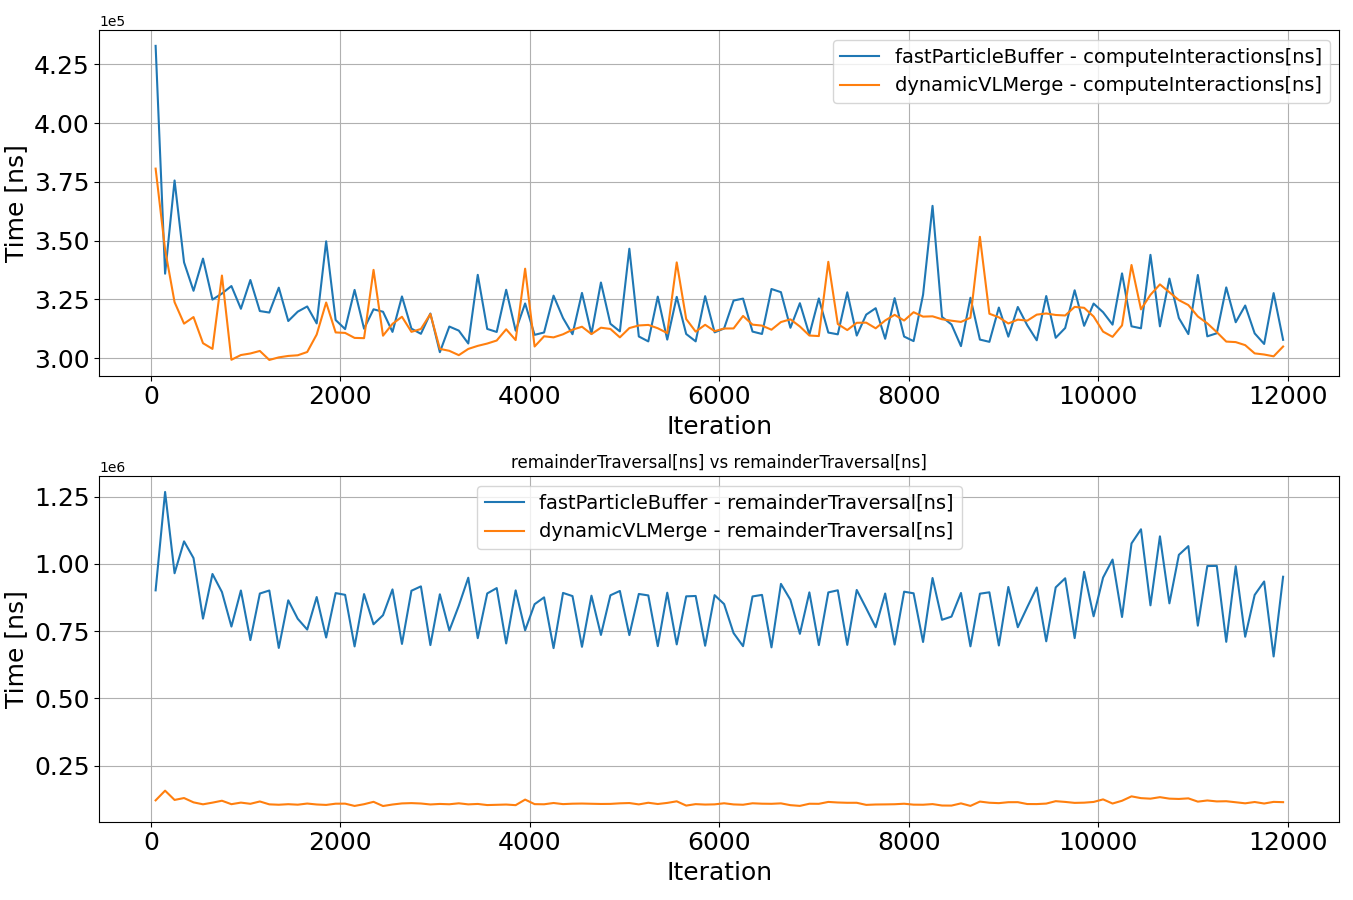
\includegraphics[width=0.9\linewidth]{graphs/explodingLiquid/normalExperiments/freq/vlc_c08inter.png}
        \vspace{-0.5em}
        \caption{\scriptsize Exploding Liquid Vlc\_c08}
        \label{fig:explodingLiquid_vlc_c08inter}
    \end{subfigure}

    \vspace{1em}
    \caption{Comparison of Compute Interactions and Remainder Traversal for Exploding Liquid Experiments}
    \label{fig:mainexplodingLiquid_inter}
\end{figure}
% ======================================================

% ============================== Iteration vs Time ==============================
\section{}
\begin{figure}[H]
\centering
% Subfigure 1
\begin{subfigure}{\linewidth}
    \centering
    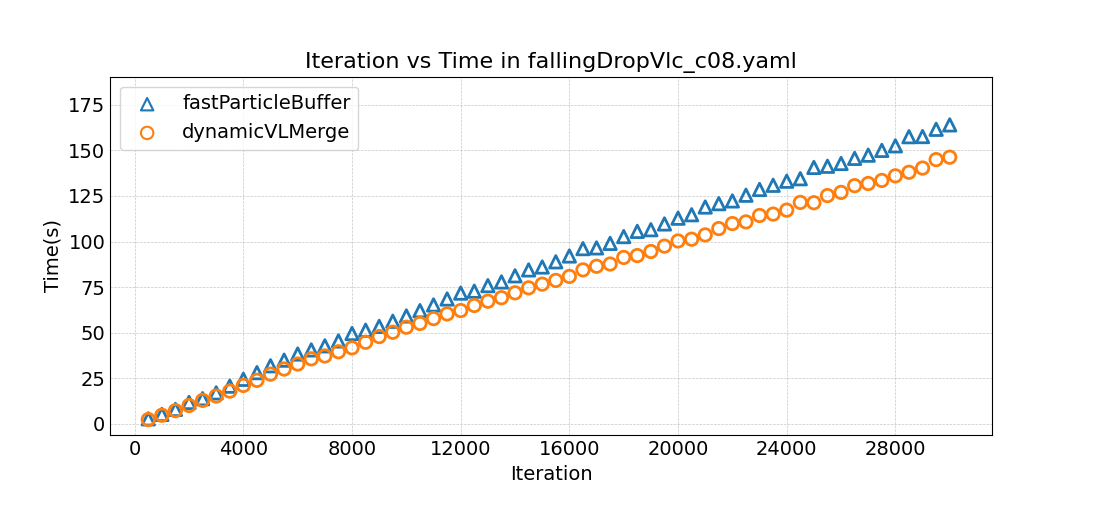
\includegraphics[width=\linewidth]{graphs/fallingDrop/normalExperiments/iter/vlcc08.png}
    \caption{Iterations vs Time for Falling Drop vlc\_c08}
    \label{fig:fallingDrop}
\end{subfigure}

% Subfigure 2
\begin{subfigure}{\linewidth}
    \centering
    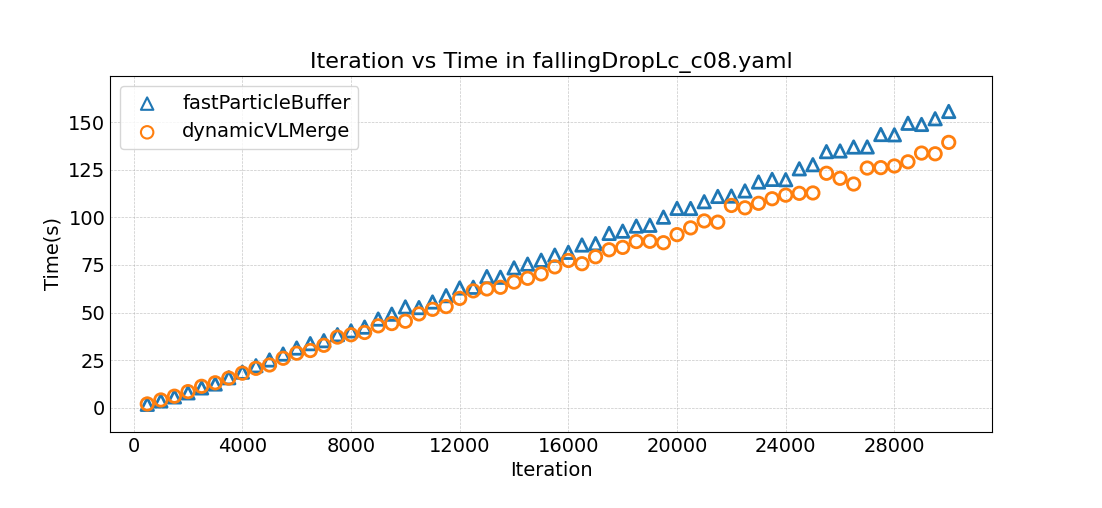
\includegraphics[width=\linewidth]{graphs/fallingDrop/normalExperiments/iter/lcc08.png}
    \caption{Iterations vs Time for Falling Drop lc\_c08}
    \label{fig:explodingLiquid}
\end{subfigure}

\label{fig:appendixGraphs}
\end{figure}

\begin{figure}[H]\ContinuedFloat
\centering
% Subfigure 3
\begin{subfigure}{\linewidth}
    \centering
    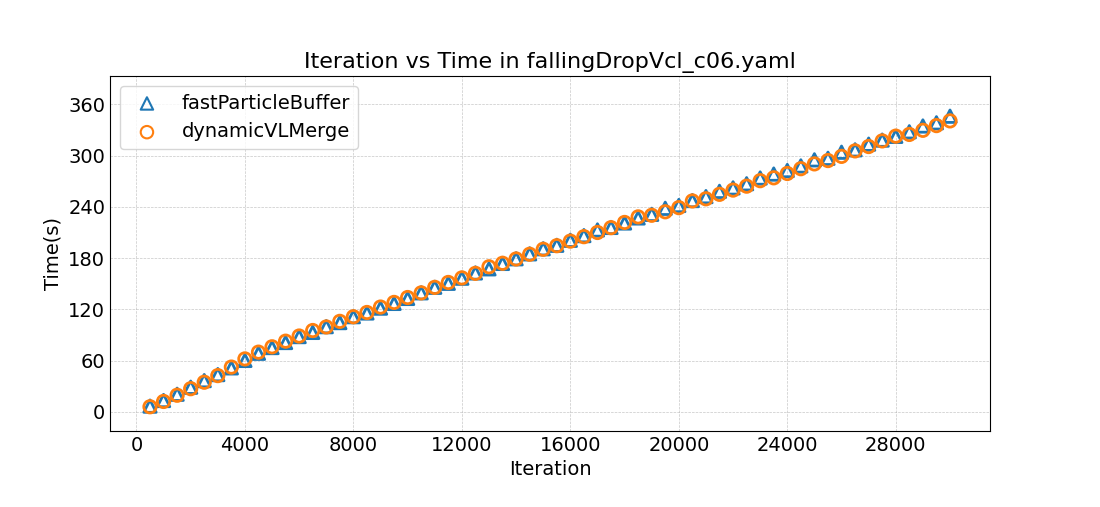
\includegraphics[width=\linewidth]{graphs/fallingDrop/normalExperiments/iter/vclc06.png}
    \caption{Iterations vs Time for Falling Drop vcl\_c06}
    \label{fig:constantVelocityCube}
\end{subfigure}
\end{figure}

\section{}
\begin{figure}[H]
\centering
% Subfigure 1
\begin{subfigure}{\linewidth}
    \centering
    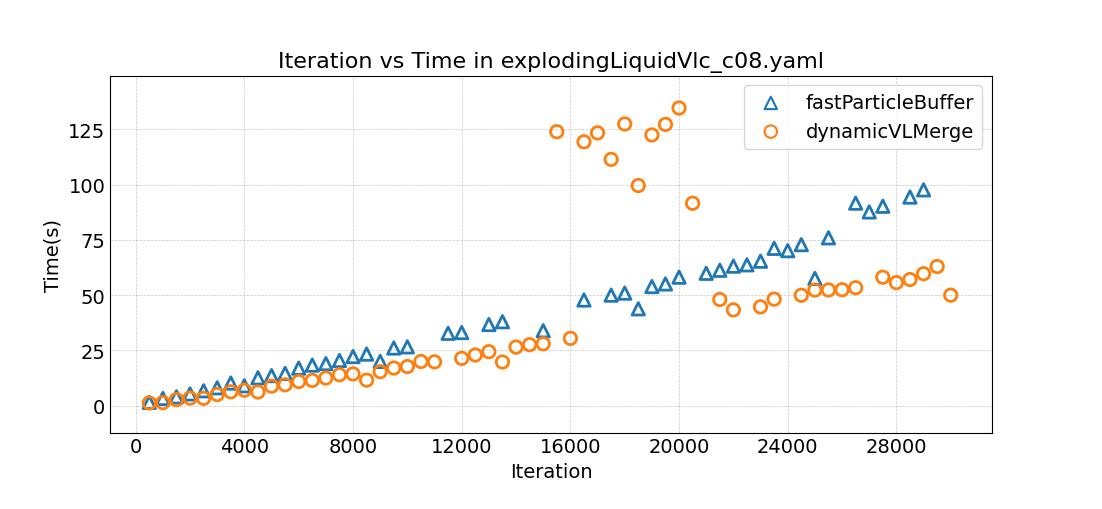
\includegraphics[width=\linewidth]{graphs/explodingLiquid/normalExperiments/iter/vlcc08.png}
    \caption{Iterations vs Time for Exploding Liquid vlc\_c08}
    \label{fig:fallingDrop}
\end{subfigure}

% Subfigure 2
\begin{subfigure}{\linewidth}
    \centering
    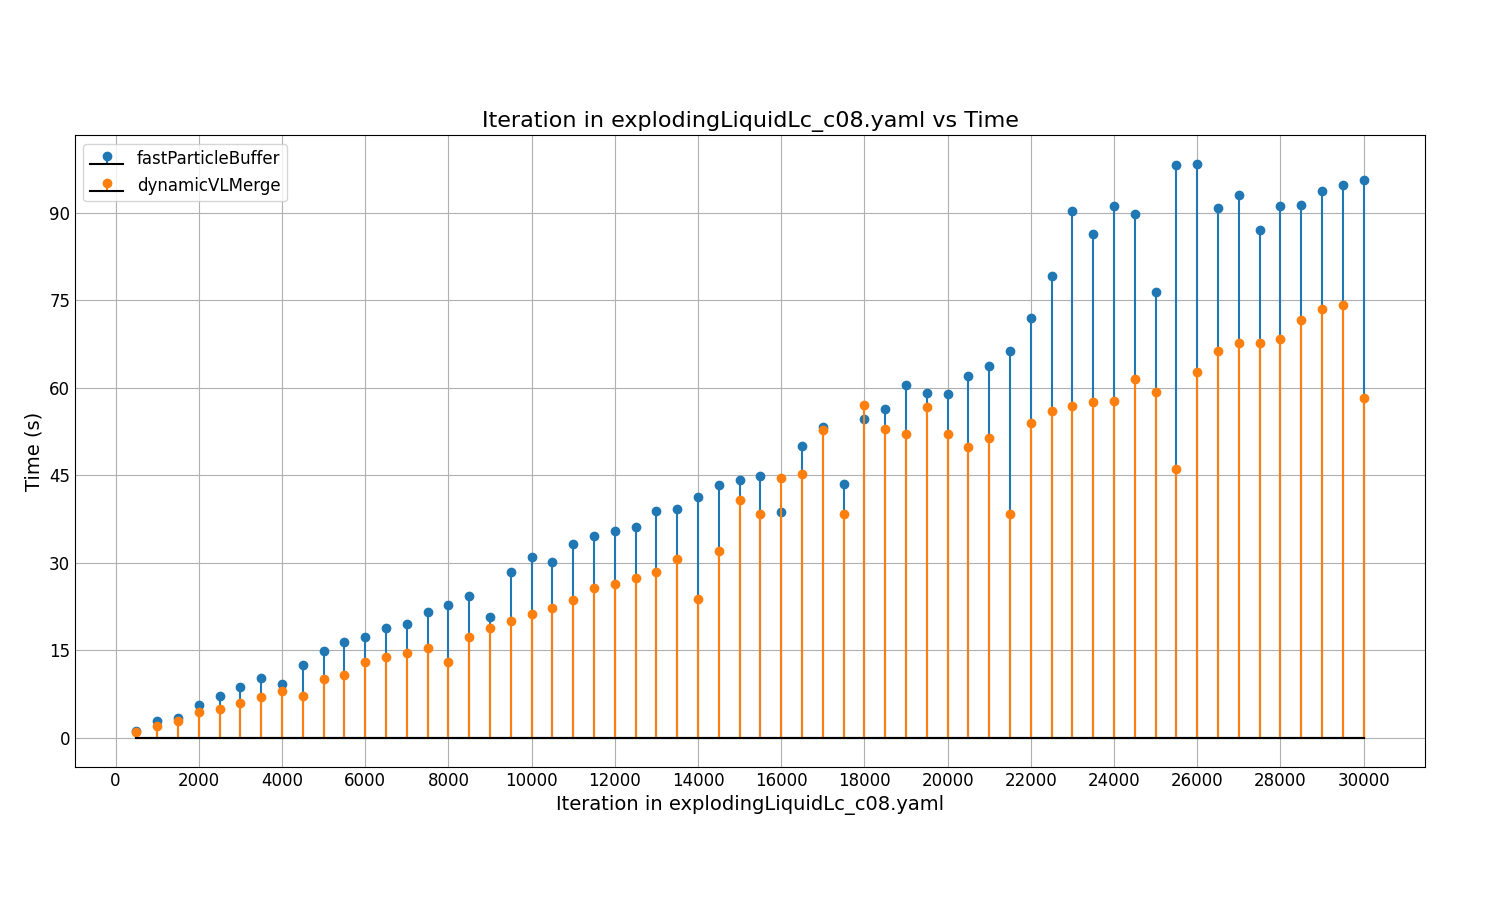
\includegraphics[width=\linewidth]{graphs/explodingLiquid/normalExperiments/iter/lcc08.png}
    \caption{Iterations vs Time for Exploding Liquid lc\_c08}
    \label{fig:explodingLiquid}
\end{subfigure}

\label{fig:appendixGraphs}
\end{figure}

\begin{figure}[H]\ContinuedFloat
\centering
% Subfigure 3
\begin{subfigure}{\linewidth}
    \centering
    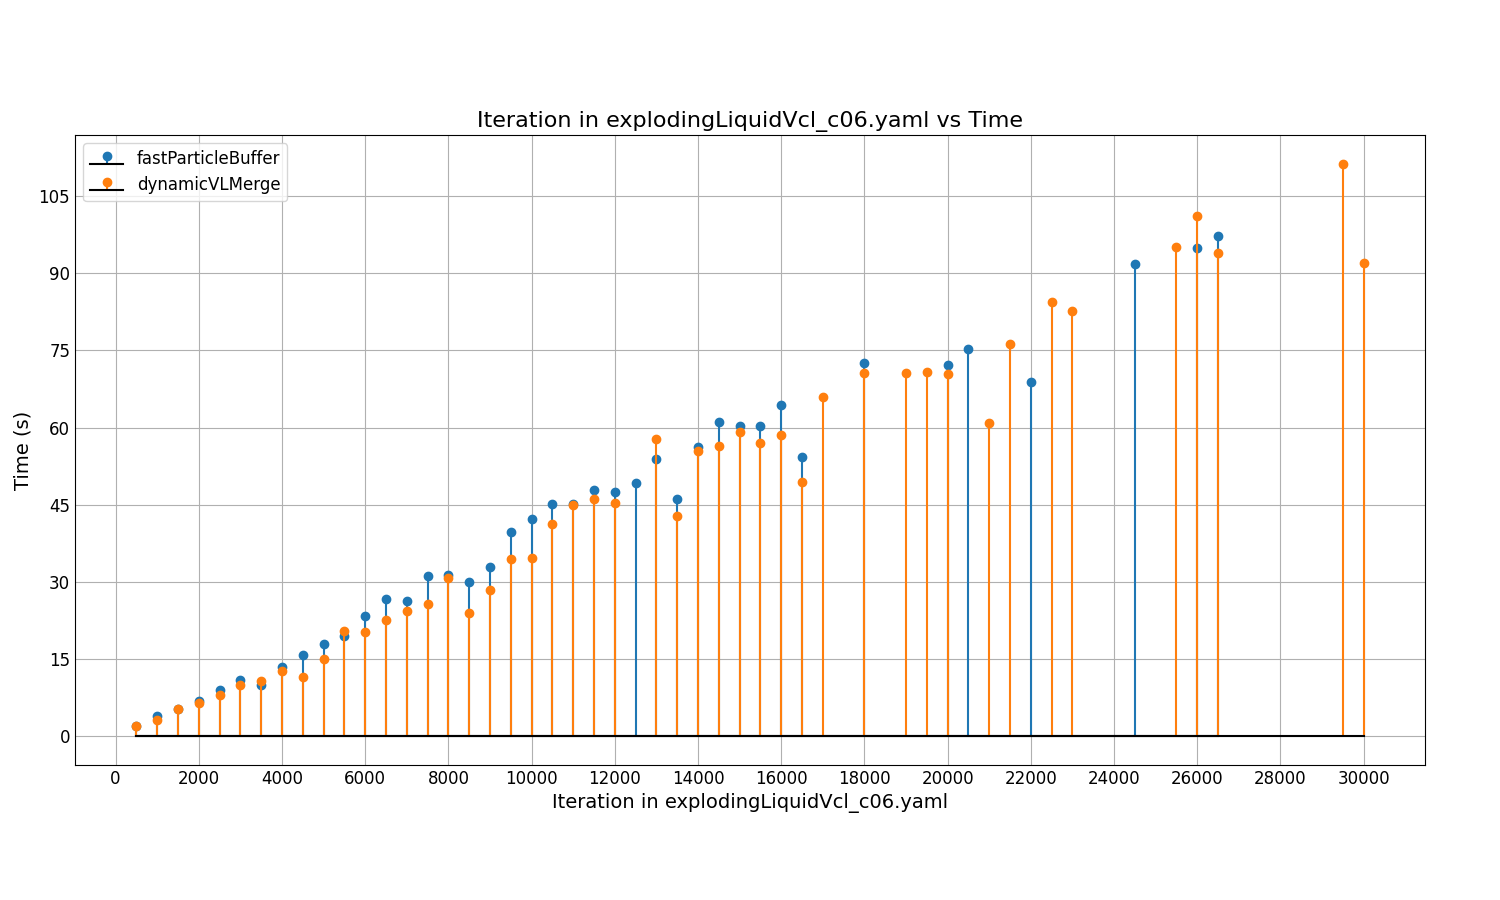
\includegraphics[width=\linewidth]{graphs/explodingLiquid/normalExperiments/iter/vclc06.png}
    \caption{Iterations vs Time for Exploding Liquid vcl\_c06}
    \label{fig:constantVelocityCube}
\end{subfigure}
\end{figure}

\section{}
\begin{figure}[H]
\centering
% Subfigure 1
\begin{subfigure}{\linewidth}
    \centering
    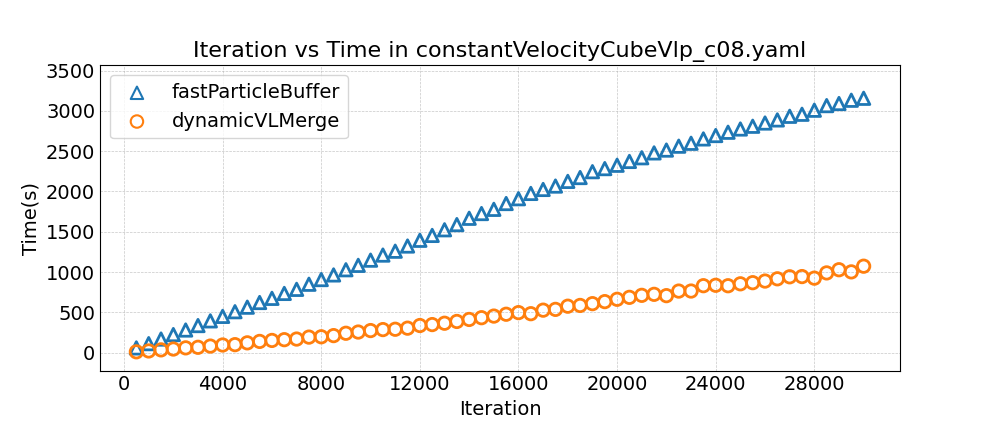
\includegraphics[width=\linewidth]{graphs/constantVelocityCube/normalExperiments/iter/vlpc08.png}
    \caption{Iterations vs Time for Constant Velocity Cube vlp\_c08}
    \label{fig:fallingDrop}
\end{subfigure}

% Subfigure 2
\begin{subfigure}{\linewidth}
    \centering
    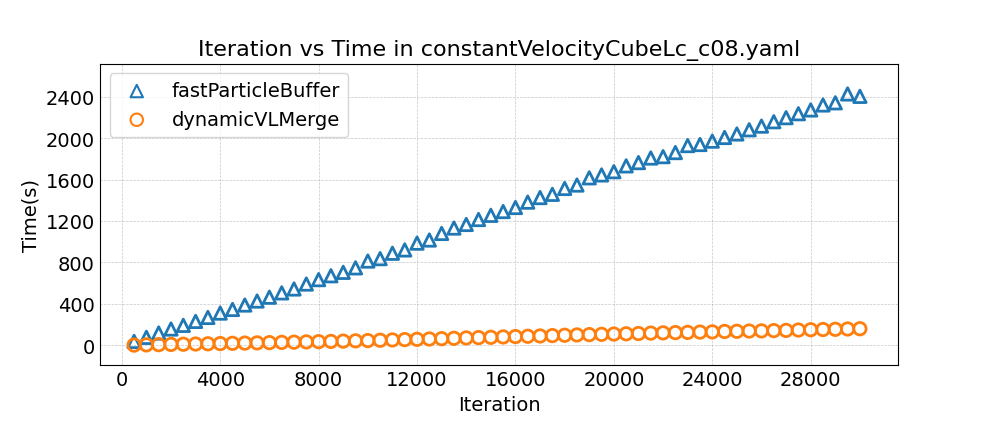
\includegraphics[width=\linewidth]{graphs/constantVelocityCube/normalExperiments/iter/lcc08.png}
    \caption{Iterations vs Time for Constant Velocity Cube lc\_c08}
    \label{fig:explodingLiquid}
\end{subfigure}

\label{fig:appendixGraphs}
\end{figure}

\begin{figure}[H]\ContinuedFloat
\centering
% Subfigure 3
\begin{subfigure}{\linewidth}
    \centering
    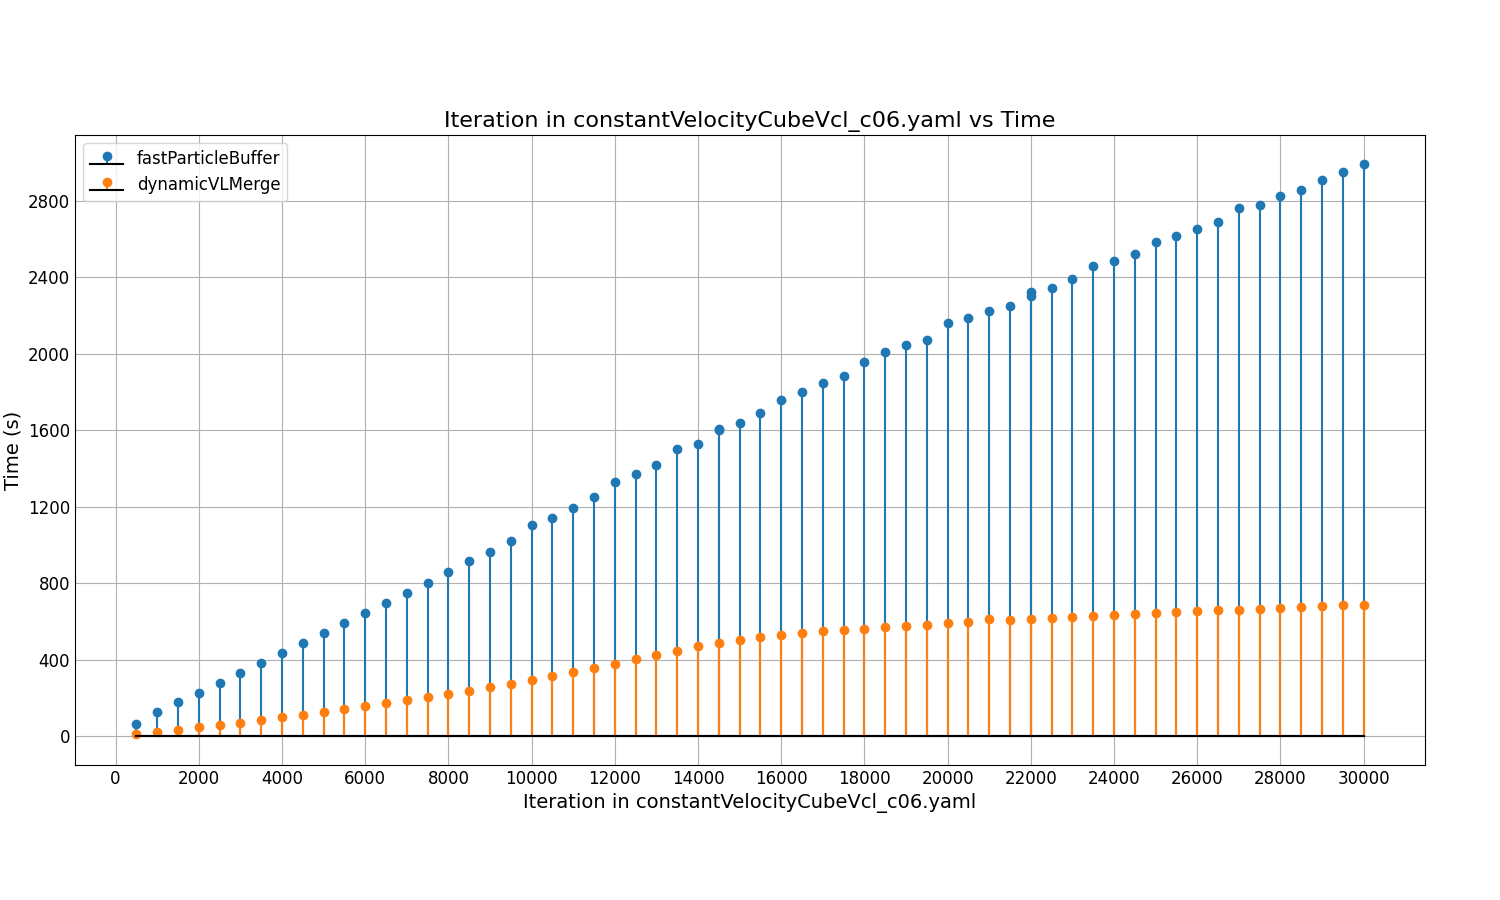
\includegraphics[width=\linewidth]{graphs/constantVelocityCube/normalExperiments/iter/vclc06.png}
    \caption{Iterations vs Time for Constant Velocity Cube vcl\_c06}
    \label{fig:constantVelocityCube}
\end{subfigure}
\end{figure}



% ======================================================



% ==================Spinodal Decomposition Equilibration ====================

\section{}
\begin{figure}[H]
\centering
% Subfigure 1
\begin{subfigure}{\linewidth}
    \centering
    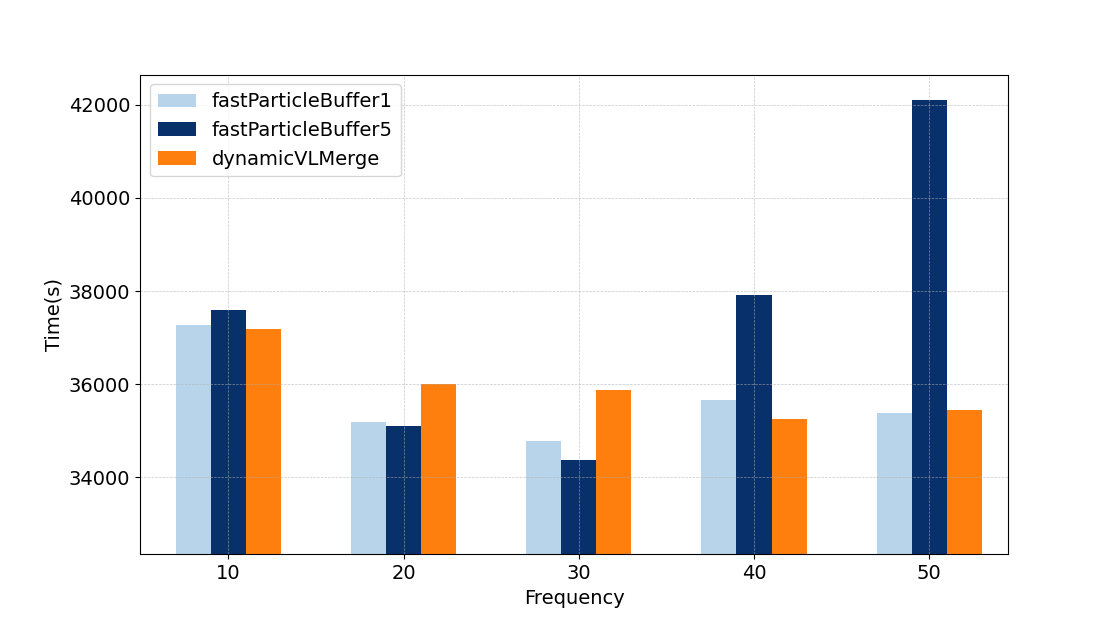
\includegraphics[width=\linewidth]{graphs/spinodalDecomposition/vlcc08.png}
    \caption{Iterations vs Time for Spinodal Decomposition vlc\_c08}
    \label{fig:fallingDrop}
\end{subfigure}

% Subfigure 2
\begin{subfigure}{\linewidth}
    \centering
    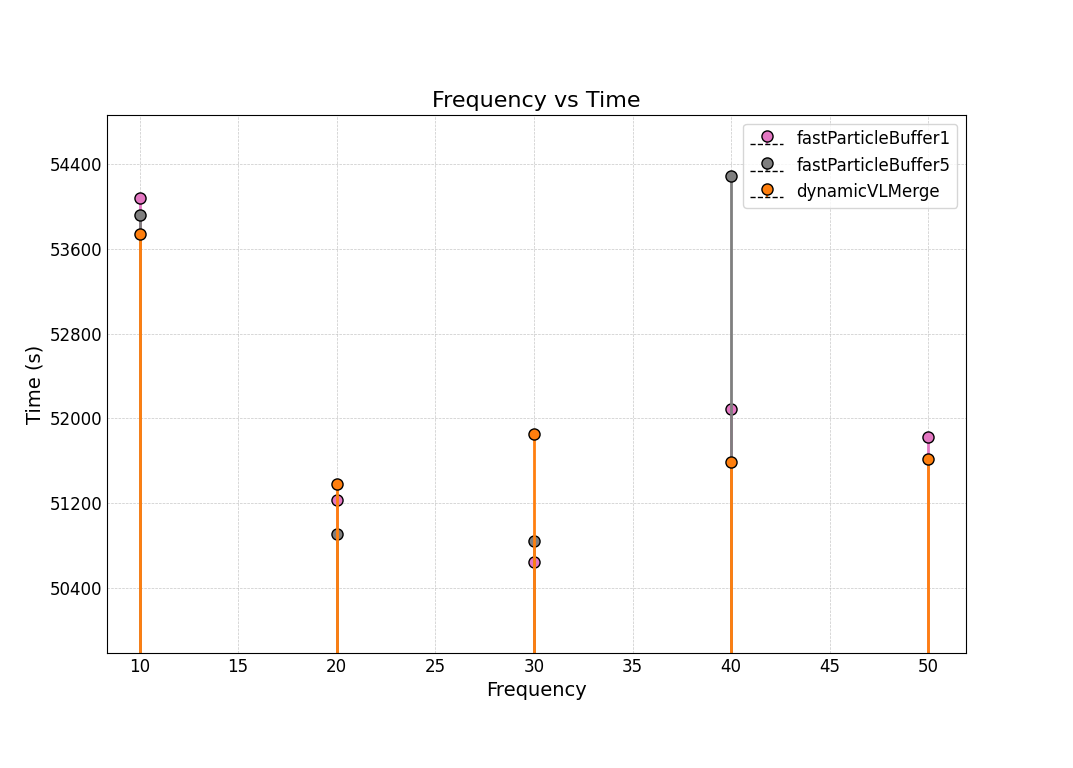
\includegraphics[width=\linewidth]{graphs/spinodalDecomposition/lcc08.png}
    \caption{Frequency vs Time for Spinodal Decomposition lc\_c08}
    \label{fig:explodingLiquid}
\end{subfigure}

\label{fig:appendixGraphs}
\end{figure}

% ======================================================


